\documentclass[landscape,final,b0paper,fontscale=0.285]{baposter}

\usepackage{calc}
\usepackage{graphicx}
\usepackage{amsmath}
\usepackage{amssymb}
\usepackage{relsize}
\usepackage{multirow}
\usepackage{rotating}
\usepackage{bm}
\usepackage{url}
\usepackage{setspace}
\usepackage{caption}
\usepackage{color}
\DeclareMathOperator*{\argmax}{argmax}


\usepackage{graphicx}
\usepackage{multicol}

%\usepackage{times}
%\usepackage{helvet}
%\usepackage{bookman}
\usepackage{palatino}

\graphicspath{{images/}{../images/}}
\usetikzlibrary{calc}

\newcommand{\SET}[1]  {\ensuremath{\mathcal{#1}}}
\newcommand{\MAT}[1]  {\ensuremath{\boldsymbol{#1}}}
\newcommand{\VEC}[1]  {\ensuremath{\boldsymbol{#1}}}
\newcommand{\Video}{\SET{V}}
\newcommand{\video}{\VEC{f}}
\newcommand{\track}{x}
\newcommand{\Track}{\SET T}
\newcommand{\LMs}{\SET L}
\newcommand{\lm}{l}
\newcommand{\PosE}{\SET P}
\newcommand{\posE}{\VEC p}
\newcommand{\negE}{\VEC n}
\newcommand{\NegE}{\SET N}
\newcommand{\Occluded}{\SET O}
\newcommand{\occluded}{o}

%%%%%%%%%%%%%%%%%%%%%%%%%%%%%%%%%%%%%%%%%%%%%%%%%%%%%%%%%%%%%%%%%%%%%%%%%%%%%%%%
%%%% Some math symbols used in the text
%%%%%%%%%%%%%%%%%%%%%%%%%%%%%%%%%%%%%%%%%%%%%%%%%%%%%%%%%%%%%%%%%%%%%%%%%%%%%%%%

%%%%%%%%%%%%%%%%%%%%%%%%%%%%%%%%%%%%%%%%%%%%%%%%%%%%%%%%%%%%%%%%%%%%%%%%%%%%%%%%
% Multicol Settings
%%%%%%%%%%%%%%%%%%%%%%%%%%%%%%%%%%%%%%%%%%%%%%%%%%%%%%%%%%%%%%%%%%%%%%%%%%%%%%%%
\setlength{\columnsep}{1.5em}
\setlength{\columnseprule}{0mm}

%%%%%%%%%%%%%%%%%%%%%%%%%%%%%%%%%%%%%%%%%%%%%%%%%%%%%%%%%%%%%%%%%%%%%%%%%%%%%%%%
% Save space in lists. Use this after the opening of the list
%%%%%%%%%%%%%%%%%%%%%%%%%%%%%%%%%%%%%%%%%%%%%%%%%%%%%%%%%%%%%%%%%%%%%%%%%%%%%%%%
\newcommand{\compresslist}{%
\setlength{\itemsep}{1pt}%
\setlength{\parskip}{0pt}%
\setlength{\parsep}{0pt}%
}

%%%%%%%%%%%%%%%%%%%%%%%%%%%%%%%%%%%%%%%%%%%%%%%%%%%%%%%%%%%%%%%%%%%%%%%%%%%%%%
%%% Begin of Document
%%%%%%%%%%%%%%%%%%%%%%%%%%%%%%%%%%%%%%%%%%%%%%%%%%%%%%%%%%%%%%%%%%%%%%%%%%%%%%

\begin{document}

%%%%%%%%%%%%%%%%%%%%%%%%%%%%%%%%%%%%%%%%%%%%%%%%%%%%%%%%%%%%%%%%%%%%%%%%%%%%%%
%%% Here starts the poster
%%%---------------------------------------------------------------------------
%%% Format it to your taste with the options
%%%%%%%%%%%%%%%%%%%%%%%%%%%%%%%%%%%%%%%%%%%%%%%%%%%%%%%%%%%%%%%%%%%%%%%%%%%%%%
% Define some colors

%\definecolor{lightblue}{cmyk}{0.83,0.24,0,0.12}
\definecolor{lightblue}{rgb}{0.145,0.6666,1}

% Draw a video
\newlength{\FSZ}
\newcommand{\drawvideo}[3]{% [0 0.25 0.5 0.75 1 1.25 1.5]
   \noindent\pgfmathsetlength{\FSZ}{\linewidth/#2}
   \begin{tikzpicture}[outer sep=0pt,inner sep=0pt,x=\FSZ,y=\FSZ]
   \draw[color=lightblue!50!black] (0,0) node[outer sep=0pt,inner sep=0pt,text width=\linewidth,minimum height=0] (video) {\noindent#3};
   \path [fill=lightblue!50!black,line width=0pt] 
     (video.north west) rectangle ([yshift=\FSZ] video.north east) 
    \foreach \x in {1,2,...,#2} {
      {[rounded corners=0.6] ($(video.north west)+(-0.7,0.8)+(\x,0)$) rectangle +(0.4,-0.6)}
    }
;
   \path [fill=lightblue!50!black,line width=0pt] 
     ([yshift=-1\FSZ] video.south west) rectangle (video.south east) 
    \foreach \x in {1,2,...,#2} {
      {[rounded corners=0.6] ($(video.south west)+(-0.7,-0.2)+(\x,0)$) rectangle +(0.4,-0.6)}
    }
;
   \foreach \x in {1,...,#1} {
     \draw[color=lightblue!50!black] ([xshift=\x\linewidth/#1] video.north west) -- ([xshift=\x\linewidth/#1] video.south west);
   }
   \foreach \x in {0,#1} {
     \draw[color=lightblue!50!black] ([xshift=\x\linewidth/#1,yshift=1\FSZ] video.north west) -- ([xshift=\x\linewidth/#1,yshift=-1\FSZ] video.south west);
   }
   \end{tikzpicture}
}

\hyphenation{resolution occlusions}
%%
\begin{poster}%
  % Poster Options
  {
  % Show grid to help with alignment
  grid=false,
  % Column spacing
  colspacing=1em,
  % Color style
  bgColorOne=white,
  bgColorTwo=white,
  borderColor=lightblue,
  headerColorOne=black,
  headerColorTwo=lightblue,
  headerFontColor=white,
  boxColorOne=white,
  boxColorTwo=lightblue,
  % Format of textbox
  textborder=roundedleft,
  % Format of text header
  eyecatcher=true,
  headerborder=closed,
  headerheight=0.1\textheight,
%  textfont=\sc, An example of changing the text font
  headershape=roundedright,
  headershade=shadelr,
  headerfont=\Large\bf\textsc, %Sans Serif
  textfont={\setlength{\parindent}{1em}},
  boxshade=plain,
%  background=shade-tb,
  background=plain,
  linewidth=2pt
  }
  % Eye Catcher
  {}
  % Title
  {\bf{Real Multi-Sense or Pseudo Multi-Sense: An Approach to Improve Word Representation}\vspace{0.1em}}
  % Authors
  {{Haoyue Shi, Caihua Li and Junfeng Hu} ~~~~~~~~~~  \{hyshi, peterli, hujf\}@pku.edu.cn \\[0.1em] {School of Electronics Engineering and Computer Science, Peking University}}
  % University logo
  {% The makebox allows the title to flow into the logo, this is a hack because of the L shaped logo.
    
\includegraphics[height=7.5em]{images/logo}
  }
%%%%%%%%%%%%%%%%%%%%%%%%%%%%%%%%%%%%%%%%%%%%%%%%%%%%%%%%%%%%%%%%%%%%%%%%%%%%%%
%%% Now define the boxes that make up the poster
%%%---------------------------------------------------------------------------
%%% Each box has a name and can be placed absolutely or relatively.
%%% The only inconvenience is that you can only specify a relative position 
%%% towards an already declared box. So if you have a box attached to the 
%%% bottom, one to the top and a third one which should be in between, you 
%%% have to specify the top and bottom boxes before you specify the middle 
%%% box.
%%%%%%%%%%%%%%%%%%%%%%%%%%%%%%%%%%%%%%%%%%%%%%%%%%%%%%%%%%%%%%%%%%%%%%%%%%%%%%
    %
    % A coloured circle useful as a bullet with an adjustably strong filling
    \newcommand{\colouredcircle}{%
      \tikz{\useasboundingbox (-0.2em,-0.32em) rectangle(0.2em,0.32em); \draw[draw=black,fill=lightblue,line width=0.03em] (0,0) circle(0.18em);}}

%%%%%%%%%%%%%%%%%%%%%%%%%%%%%%%%%%%%%%%%%%%%%%%%%%%%%%%%%%%%%%%%%%%%%%%%%%%%%%
  \headerbox{Abstract}{name=abstract,column=0,row=0}{
%%%%%%%%%%%%%%%%%%%%%%%%%%%%%%%%%%%%%%%%%%%%%%%%%%%%%%%%%%%%%%%%%%%%%%%%%%%%%%
\par
Previous researches have shown that learning multiple representations for polysemous words can improve the performance of word embeddings on many tasks. However, this leads to another problem. Several vectors of a word may actually point to the same meaning, namely pseudo multi-sense. 
\par
We introduce the concept of pseudo multi-sense, and then propose an algorithm to detect such cases. With the consideration of the detected pseudo multi-sense cases, we try to refine the existing word embeddings to eliminate the influence of pseudo multi-sense. Moreover, we apply our algorithm on previous released multi-sense word embeddings and tested it on artificial word similarity tasks and the analogy task. The result of the experiments shows that diminishing pseudo multi-sense can improve the quality of word representations. Thus, our method is actually an efficient way to reduce linguistic complexity for computer's natural language understanding. 
   \vspace{0.3em}
 }

%%%%%%%%%%%%%%%%%%%%%%%%%%%%%%%%%%%%%%%%%%%%%%%%%%%%%%%%%%%%%%%%%%%%%%%%%%%%%%
  \headerbox{Pseudo Multi-Sense Detection}{name=detection,column=1,row=0}{
%%%%%%%%%%%%%%%%%%%%%%%%%%%%%%%%%%%%%%%%%%%%%%%%%%%%%%%%%%%%%%%%%%%%%%%%%%%%%%
\noindent\textbf{\large Domain Similarity}
\par To determine the domain of a sense given the multi-sense word embeddings, we can intuitively define the probability that the $k^{th}$ sense of word $w$ belongs to domain $d$ as 
\begin{equation} \label{pdomain}
P_D(w, k, d) \propto  {\sum_{w' \in NN(w, k)} D(p(w'), d)} \nonumber
\end{equation}
where $NN(w,k)$ is the nearest neighbors of the $k^{th}$ sense of word $w$ in the given word embeddings, $p(w')$ is the protocol representation of word $w'$, $D(p(w'), d)$ is the sum probability that domain $d$ appears in all synsets of $p(w')$ in WordNet(\cite{wordnet}) provided by Extended WordNet Domain. Then we can compute the domain similarity between the $k^{th}$ and the $l^{th}$ sense of word $w$ by
\begin{equation}
Sim_D(w,k,l) = \frac 1n|TopN(P_D,w,k,n) \cap TopN(P_D,w,l,n)| \nonumber
\end{equation}
\noindent\textbf{\large Semantic Similarity}
\par 
Analogously, we can define semantic similarity.
\begin{equation} \label{simh}
Sim_H(w,k,l) = \frac 1n|TopN(P_H,w,k,n) \cap TopN(P_H,w,l,n)| \nonumber
\end{equation}
where 
\begin{equation} \label{phyper}
P_H(w, k, h) \propto \frac{1}{d(w,h)} {\sum_{w' \in NN(w, k)} H(p(w'), h)} \cdot \frac{1}{d(p(w'),h)} \nonumber
\end{equation}
\noindent\textbf{\large Overall Similarity}
\par
We sum the domain similarity and the semantic similarity to get the overall similarity of two sense. 
\begin{equation} \label{simall}
Sim(w,k,l) = Sim_D(w,k,l) + Sim_H(w,k,l) \nonumber
\end{equation}
\par
With a development dataset, we set a threshold $\theta$ for regarding two senses of a word as pseudo multi-sense.
\\~\\
\noindent\textbf{\large Detected Samples}
\par 
Here shows nearest neighbors three "senses" of word {\sl rock} from the released vectors in \cite{neelakantan}. 
\begin{itemize}
\item {\color{blue}\textbf{rock$_1$}: metal, rippling, psychedelia, bands, pop}
\item {\color{orange}\textbf{rock$_2$}: sand, rocks, butte, ash, sandy, cedar}
\item {\color{blue}\textbf{rock$_3$}: hip, indie, hop, reggae, roll, rock/metal}
\end{itemize}
Our algorithm shows that rock$_1$ and rock$_3$ are likely to be pseudo multi-sense, while rock$_2$ has a different meaning with them. 
   \vspace{0.3em}
  }

%%%%%%%%%%%%%%%%%%%%%%%%%%%%%%%%%%%%%%%%%%%%%%%%%%%%%%%%%%%%%%%%%%%%%%%%%%%%%%
\headerbox{Pseudo Multi-Sense Elimination}{name=elimination,column=2,span=2,row=0}{
  %%%%%%%%%%%%%%%%%%%%%%%%%%%%%%%%%%%%%%%%%%%%%%%%%%%%%%%%%%%%%%%%%%%%%%%%%%%%%%
	\begin{center}
      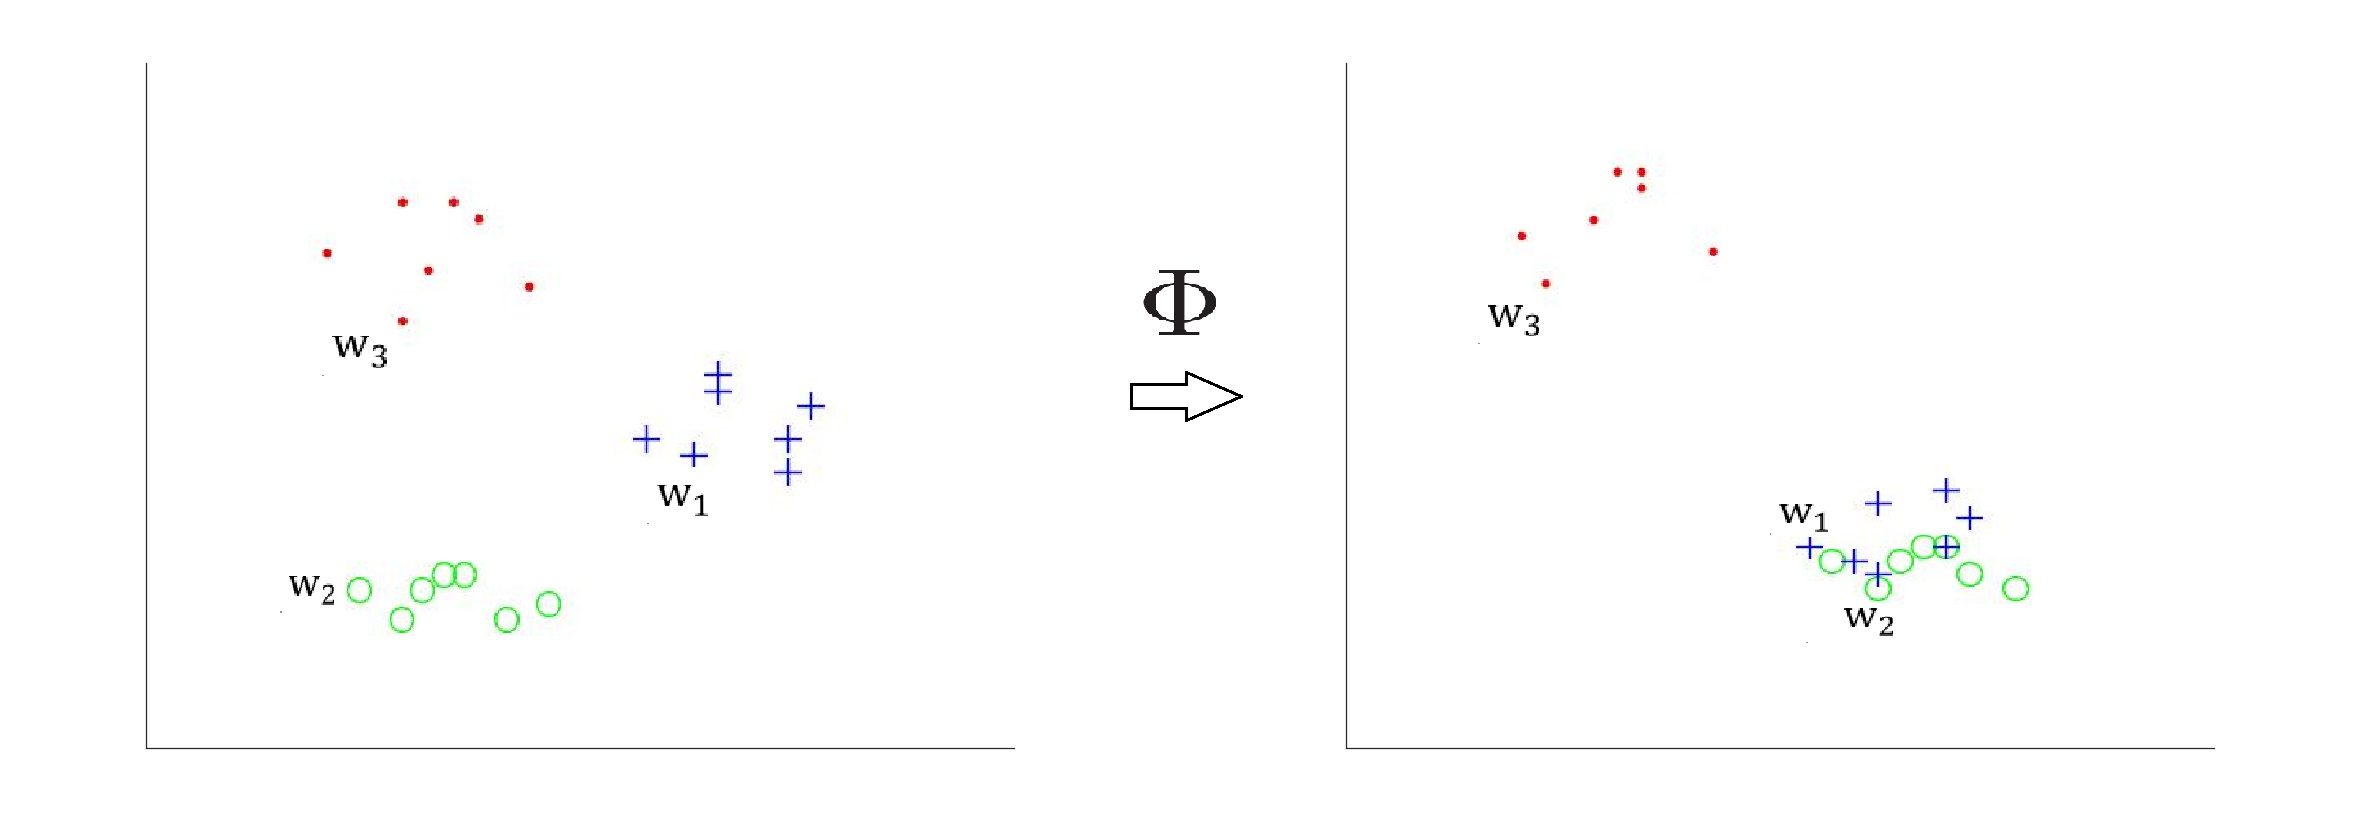
\includegraphics[width=0.5\linewidth]{orig}
	  \\ \vspace{-0.8em}
	  \captionof{figure}{How the global transform matrix works. In the case, w$_1$, w$_2$ and $w_3$ are senses produced by previous word embedding algorithm automatically. We detect w$_1$ and w$_2$ have the same meaning in fact while w$_3$ has a different meaning.}
	  \end{center}
      \begin{multicols}{2}
    Having the existing word embeddings, assume that we have a detected pseudo multi-sense group $G = \{w_{k_1}, w_{k_2}, ... , w_{k_n}\}$, in which $w_{k_1}, w_{k_2}, ... , w_{k_n}$ are senses of word $w$, taking the same meaning. Thus, we can find a representative vector for the group. Let $v_s(w,k_i)$ be the corresponding vectors of $w_{k_i}$, and $v_r(G)$ be the representative vector for the group $G$. Such vector $v_r(G)$ can be randomly chosen from $\{v_s(w,k_1), v_s(w,k_2), ..., v_s(w,k_n)\}$, or simply the mean vector of them. Other methods to compute $v_r(G)$ are also worth trying if reasonable. 
	\par
	Assume there is a transition matrix, by which for all pseudo multi-sense group $G$, $\forall w_{k_i} \in G$, $v_{w_{k_i}}$ can be projected to $v_r(G)$. In other words, we suggest that there exists a global matrix $\Phi$, for any given pseudo multi-sense group $G = \{w_{k_1}, w_{k_2}, ... , w_{k_n}\}$ and its representative vector $v_r(G)$, we have
\begin{equation}
v_r(G) = \Phi * v_s(w, k_i), \forall w_{k_i} \in G, \forall G \nonumber
\end{equation}
	Thus we can eliminate pseudo multi-sense by applying $\Phi$ to the original vector space.
      \end{multicols}
      \vspace{-0.6em}
}
%%%%%%%%%%%%%%%%%%%%%%%%%%%%%%%%%%%%%%%%%%%%%%%%%%%%%%%%%%%%%%%%%%%%%%%%%%%%%%
  \headerbox{References}{name=references,column=0,span=3,above=bottom}{
%%%%%%%%%%%%%%%%%%%%%%%%%%%%%%%%%%%%%%%%%%%%%%%%%%%%%%%%%%%%%%%%%%%%%%%%%%%%%%
    \smaller
    \bibliographystyle{acl}
    \renewcommand{\section}[2]{\vskip 0.05em}
      \begin{thebibliography}{1}\itemsep=-0.01em
      \setlength{\baselineskip}{0.4em}
      \bibitem{huang}
        Eric H Huang, Richard Socher, Christopher D Manning, and Andrew Y Ng.
        \newblock  Improving word representations via global context and multiple word prototypes.
        \newblock In {\em ACL 2012}
      \bibitem{neelakantan}
		Arvind Neelakantan, Jeevan Shankar, Alexandre Passos, and Andrew McCallum.
		\newblock  Efficient non-parametric estimation of multiple embeddings per word in vector space.
        \newblock In {\em ACL 2014}
	  \bibitem{wordnet}
		George A Miller
		\newblock Wordnet: a lexical database for English.
		\newblock 1995, Communications of the ACM.
	  \bibitem{exwordnetdomain}
	  Aitor González, German Rigau, and Mauro Castillo. 
	  \newblock A graph-based method to improve wordnet domains.
	  \newblock In {\em ICITPCL 2012}
      \end{thebibliography}
   \vspace{0.3em}
  }
%%%%%%%%%%%%%%%%%%%%%%%%%%%%%%%%%%%%%%%%%%%%%%%%%%%%%%%%%%%%%%%%%%%%%%%%%%%%%%
  \headerbox{Acknowledgement}{name=references,column=3,aligned=references,above=bottom}{
%%%%%%%%%%%%%%%%%%%%%%%%%%%%%%%%%%%%%%%%%%%%%%%%%%%%%%%%%%%%%%%%%%%%%%%%%%%%%%
~\\[1em]
This work is supported by the National Natural Science Foundation of China (grant No.61472017, M1552004).
   \vspace{0.3em}
  }
%%%%%%%%%%%%%%%%%%%%%%%%%%%%%%%%%%%%%%%%%%%%%%%%%%%%%%%%%%%%%%%%%%%%%%%%%%%%%%
\headerbox{Experiments}{name=experiments,column=2,span=2,row=0,below=elimination,above=references}{
  %%%%%%%%%%%%%%%%%%%%%%%%%%%%%%%%%%%%%%%%%%%%%%%%%%%%%%%%%%%%%%%%%%%%%%%%%%%%%%
    \begin{multicols}{2}
	\begin{center}
      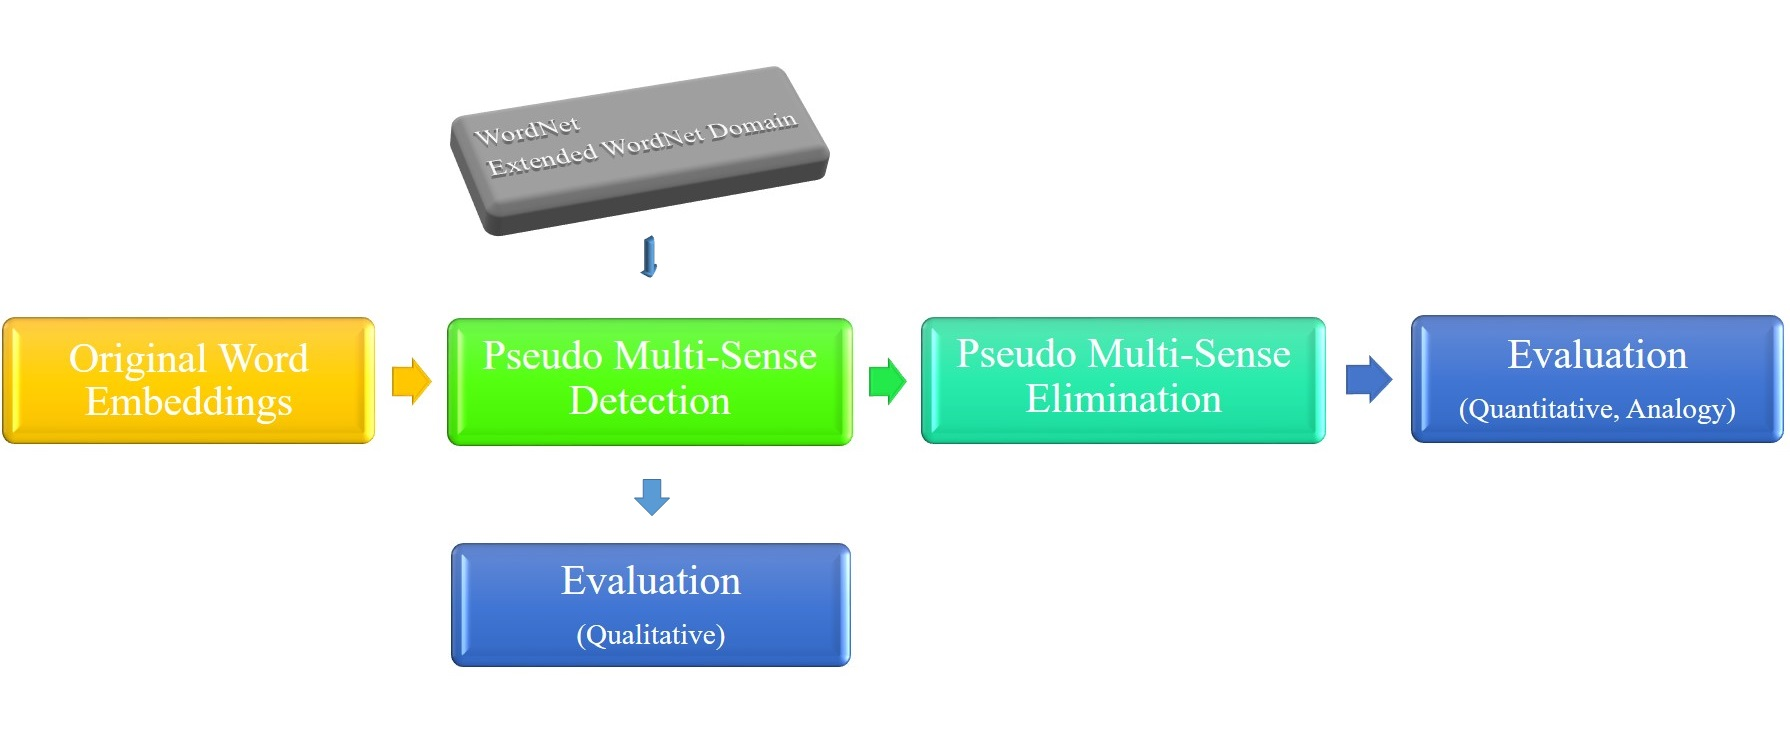
\includegraphics[width=\linewidth]{flow}
	  \\ \vspace{-0.8em}
	  \captionof{figure}{The pipeline of our experiment.}
	  \end{center}
\noindent \textbf{\large Local Word Similarity}
\par
We evaluate our algorithm by applying it to the word vectors released by Huang et al.(\cite{huang}) and Neelakantan et al.(\cite{neelakantan}), and comparing the word similarity on SCWS dataset(\cite{huang}). The experiment shows that our algorithm gains a significant improvement on localSim metric, which is defined as 
\begin{equation}
localSim(w,w') = s(v_s(w,k), v_s(w',k'))\nonumber
\end{equation}
where $k = \mathop{\argmax}_i P(w,c,i)$, $k' = \mathop{\argmax}_{i'} P(w',c',i')$.
\begin{center}
 \begin{tabular}{|c|cc|}
 \hline
 \multirow{1}{*}{\textbf{Original Vectors}} &\multicolumn{2}{c|}{\textbf{localSim}} \\
\textbf{(Model)} & orig & trans \\
 \hline 
 Huang et al.  & 26.1 & \textbf{37.6} \\
 MSSG 50d & 49.2 &\textbf{53.2} \\
 MSSG 300d & 57.3 &\textbf{62.2}\\
 \hline
 \end{tabular}
 \captionof{table}{The performance of the original vectors and that of the vectors after transformation, on localSim metric.}
\end{center}
\noindent \textbf{\large Analogy}
\par
Analogy task evaluate the performance of word vectors on quadruples $(a,b,c,d)$ with the equation $v(a)-v(b) = v(c)-v(d)$. The quadruples can be (Beijing, China, Paris, France), or (great,greater,tough,tougher) etc. The experiment shows that our pseudo multi-sense eliminating algorithm improves the vectors' performance on analogy task.
 \begin{center}
 \begin{tabular}{|c|cc|cc|}
 \hline
 \multirow{1}{*}{\textbf{Model}} &\multicolumn{2}{c}{\textbf{Semantic}} & \multicolumn{2}{|c|}{\textbf{Syntactic}}  \\
 & orig & trans & orig & trans \\
 \hline 
 Huang et al. & 52.8 & \textbf{53.5} & 53.5 & \textbf{56.1}\\
 MSSG 50d &  75.8 & \textbf{77.5}  & 85.2 & \textbf{88.0}\\
 MSSG 300d & 92.0 & \textbf{93.1} & 93.3& \textbf{94.5}\\
 \hline
 \end{tabular}
 \captionof{table}{\label{analogy} Evaluation result on analogy task. }
 \end{center}
\end{multicols}
   \vspace{0.0em}
  }
%%%%%%%%%%%%%%%%%%%%%%%%%%%%%%%%%%%%%%%%%%%%%%%%%%%%%%%%%%%%%%%%%%%%%%%%%%%%%%
  \headerbox{Pseudo Multi-Sense}{name=pseudo multi-sense,column=0,below=abstract,bottomaligned=experiments}{
%%%%%%%%%%%%%%%%%%%%%%%%%%%%%%%%%%%%%%%%%%%%%%%%%%%%%%%%%%%%%%%%%%%%%%%%%%%%%%
\par
Polysemous words are ubiquitous in natural languages. For example, in the following two sentences, the word {\sl star} has different meanings, leaving all metaphorical considerations aside.
\begin{spacing}{-0.5} \end{spacing}
\begin{itemize}\itemsep -2pt
\item She is a famous movie \textbf{star}.
\item That small \textbf{star} is brightest. 
\end{itemize}
\par
\begin{spacing}{0.5} \end{spacing}
Some previous approaches have learned multiple embeddings to represent different senses of a word, discriminating the senses by their context, related syntax and topics. However, this leads to another problem. The methods may embed one sense to multiple vectors by mistake. We call such cases \textbf{pseudo multi-sense}. 
\par
Consider three different representations of word {\sl bear} released by \cite{neelakantan}. We show 9 nearest neighbors for each representation. Words clearly related to the domain {\sl animals} are bolded.
\begin{spacing}{-0.5} \end{spacing}
\begin{itemize} \itemsep -2pt
\item emerald, \textbf{bears}, \textbf{three-toed}, \textbf{snake}, \textbf{periwinkle}, \textbf{ruffed}, \textbf{hoopoe}, distinctive, unmistakable
\item \textbf{bird}, \textbf{wolf}, arrow, \textbf{pelican}, emerald, canyon, diamond, \textbf{buck}, \textbf{deer}
\item pride, lady, hide, king, gift, crane, afflict, promise, reap
\end{itemize}
\begin{spacing}{0.5} \end{spacing}
We could infer that the first two representations are likely to have the same meaning, namely they two are likely to form a pseudo multi-sense case. But the last representation may have different meaning with them (real multi-sense).
   \vspace{0.3em}
  }
%%%%%%%%%%%%%%%%%%%%%%%%%%%%%%%%%%%%%%%%%%%%%%%%%%%%%%%%%%%%%%%%%%%%%%%%%%%%%%

\end{poster}

\end{document}
